% !TEX root = ../thesis.tex

\chapter{Modelling motion on the \textsc{er}}\label{sec:modelling}

The messy behaviour of Aβ molecules we saw in \cref{sec:data_analysis} by the analysis of \tsc{SPT} data suggests a new hypothesis. The complex and delocalised dynamics that we found may involve active transport on the \emph{endoplasmic reticulum}, a network like organelle supporting various functions encompassing protein folding and redistribution. While it is known that the \tsc{ER} is acts as an active transportation network, it is not possible to find a directionality and the dynamics of such transport mechanism remains not clear\mcite{nehls2000dynamics}.
In a recent work, \citeauthor{holcman2018single}\mcite{holcman2018single} have shown that particles moving on the \tsc{ER} follow a two-state process, characterised by alternation of a high-velocity directed motion state associated to flow in the network tubules and a low-velocity diffusing state associated to the nodes. This kind of behaviour, with particles jumping between areas of slow motion, resembles the results the analysis performed in \cref{sec:full_picture}, motivating the hypothesis that transport of Aβ is linked to the \tsc{ER}.

As the inner workings of the \tsc{ER} are not known, it would be difficult to directly compare the the results of \cref{sec:data_analysis} to the \tsc{ER} dynamics. How are molecules redistributed in the \textsc{er}? Which timescale characterise this transport process? First, we have to understand how this network works. Thus, in this chapter we make a step back and we focus on a model of motion on the \tsc{ER}, building on the results of \citeauthor{holcman2018single}, and presenting results of numerical simulations to understand the model characteristics.

\begin{figure}[t!]
  \sidecaption{The endoplasmic reticulum of a \tsc{HEK 293T} cell imaged by fast SIM.\label{fig:er}}
  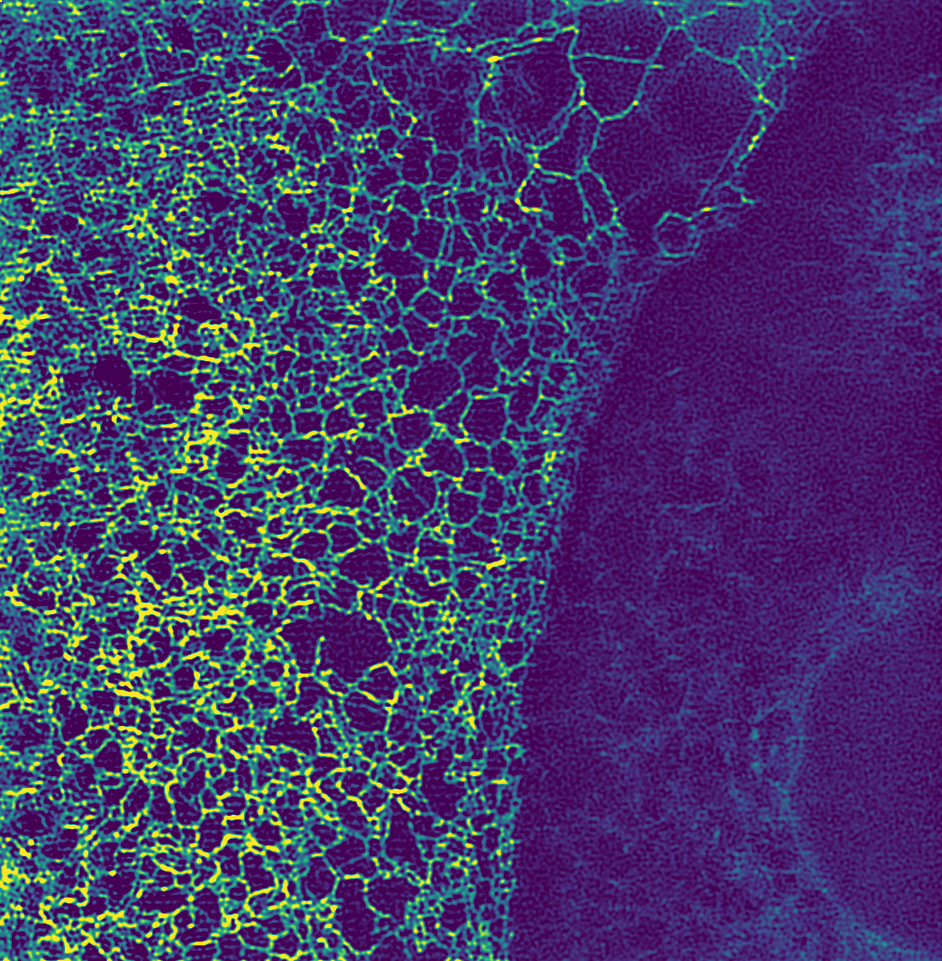
\includegraphics[width=\textwidth]{er.png}
\end{figure}

\section{Active network model}

The \textsc{er} is an organelle that spans from the nuclear envelope to the cell periphery. It has a fundamental role in the production, maturation and trafficking of proteins and lipids. A recent study based on super resolution imaging\mcite{ls_er} has revealed hat its structure is made almost exclusively of tubules at varying densities. The tubules are usually connected by three-way junctions at roughly 120 degrees\mcite{terasaki1986microtubules} (see also \cref{fig:er}). Since we only have 2 dimensional images we will refer to a planar representation of the \tsc{ER} network. This approximation is jutified by the fact that in many kind of cells the \tsc{ER} is very thin with respect to its width. Given its regular three-way junctions, the simpler planar graph representing the \tsc{ER} is an hexagonal lattice.

Some characteristics of motion on the \tsc{ER} has been recently described through the analysis of \tsc{SPT} trajectories\mcite{holcman2018single}. First, luminal proteins follow distinct transport mechanisms depending on topology: they move at fast velocity along the network tubules, and they instead move with dominant diffusive component while inside the junctions. Moreover, the luminal flow along tubules was observed to invert its direction at random time, possibly due to tubule constrictions. We introduce a model of motion that takes into account these effects.

We consider a transported molecule as a random walker on a directed graph, where edges invert their direction at a Poissonian rate ($\lambda$). Each edge will keep a directionality for an exponential time (timescale $\tau_{switch} = \frac{1}{\lambda}$), then reverse it, and so on and so forth. Moreover, the random walker spends an exponential time in each node (with timescale $\tau_{node}$). This takes into account the time required to escape from a node, given the diffusive motion inside the junction\mcite{net}. After the waiting in the node, the walker jumps randomly through one of the available outward directed edges and continues its travel. If all the edges happen to be directed inwards, the particle cannot escape and has to wait another exponential time in the node. An example of the network model is shown in figure \ref{fig:model}

\begin{figure}
  \sidecaption{Active network model. Particles diffuse inside the junctions and quickly jump along the edges. The direction of the edges alternates with rate $\lambda$ and the particles take an exponential time to escape from a junction by Brownian motion (timescale $\tau_{node}$). A trapped state (no outward flux from a junction) is marked by the dashed red rectangle.\label{fig:model}}
  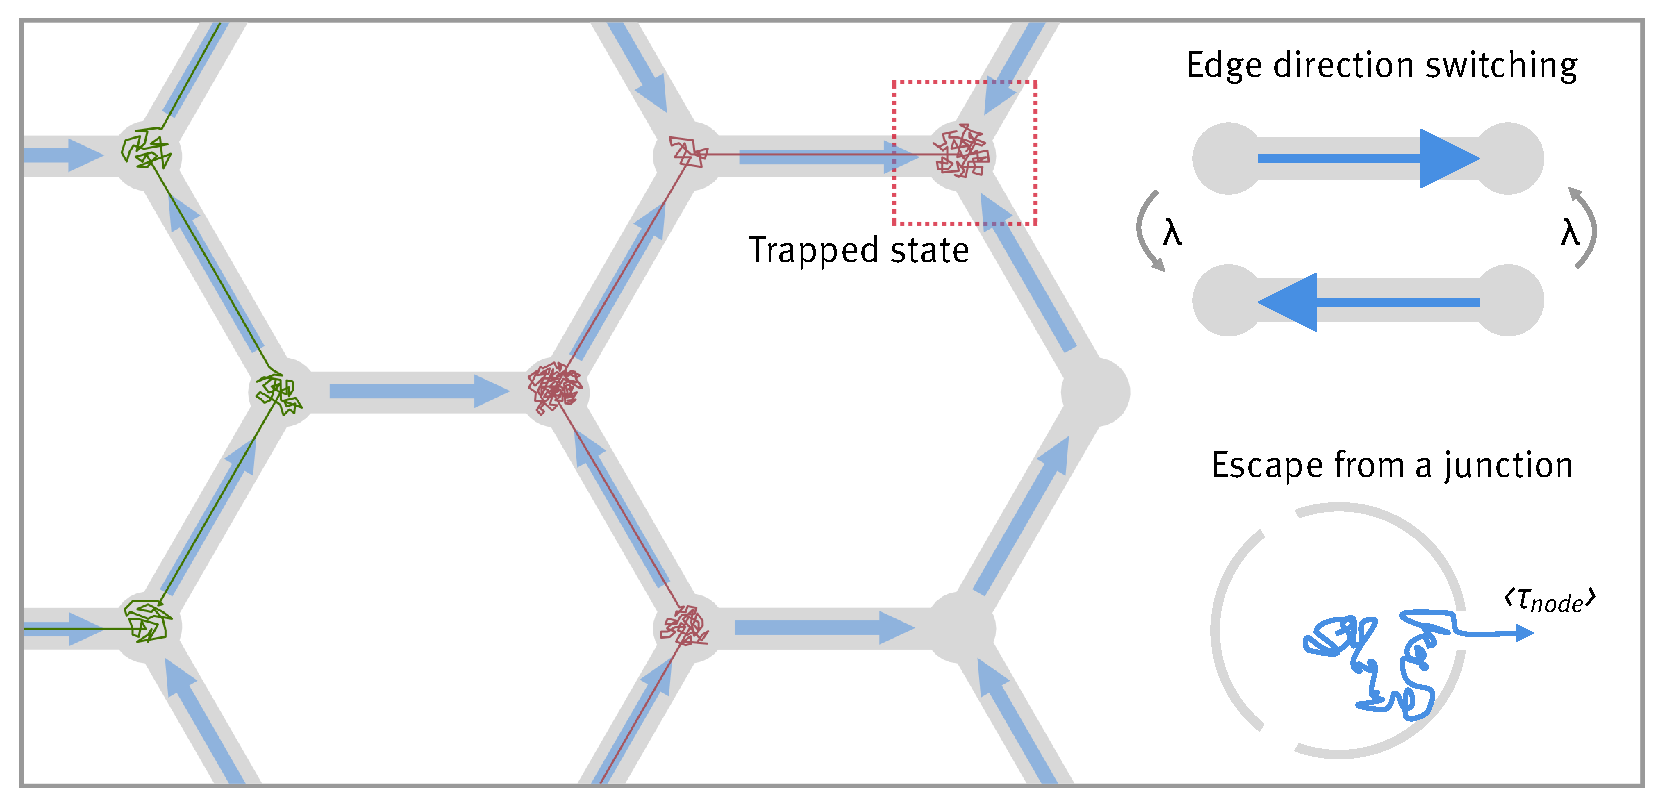
\includegraphics[width=\textwidth]{er/3_model.eps}
\end{figure}

\section{Timescale of transport}

We evaluate now the timescale of the transport on an active network. We consider two timescales that have important biological implications: the mean first passage time (\tsc{mfpt}) through a given node for a single particle and the average time required for the first particle of a group to reach a given node. This second case models an activation process where many particles are released from a source but one is sufficient to activate a receptor located in a far away node.

\subsection{Mean first passage time}

Considering a particle moving on graph starting from node $S$, the \emph{first passage time} (or \emph{hitting time}) for node $T$ is the time at which the particle first hits the target $T$. More formally,
\begin{equation}
  \tau_{S \to T}(x) = \inf \left\{ t: x(t) = T \mid x(0) = S \right\}
\end{equation}
where $x(t)$ denotes the location of the particle at time $t$.
It follows that, if $x(t)$ describes a stochastic motion, we can define the mean first passage time as
\begin{equation}
  \bar{\tau}_{S \to T} = \mathbb{E}_x\left[\tau_{S \to T}(x) \mid x(0) = S\right]
\end{equation}
where the expectation is taken over many realisations of the process.


\subsection{Extreme statistics for passage time}

We now consider the case of $N$ particles moving simultaneously on the network, all starting at the same time from the same source node $S$. In this case, we are interested in knowing the average time required for the first among the $N$ particles to hit the target $T$. Again, this is a common situation in biological systems, where a single particle may be sufficient to activate a receptor (for example, in a synapse). We define this as the minimum hitting time among N independent processes:
\begin{equation}
  \tau^{ex}_{S \to T}(N) = \min \left\{ \tau_{S \to T}(x_1), \tau_{S \to T}(x_2), \dots, \tau_{S \to T}(x_N) \right\}
\end{equation}
We can then take the average over many realisations of this multiple-particle process to define
\begin{equation}
  \bar{\tau}^{ex}_{S \to T}(N) = \mathbb{E}_{\{x_1, x_2, \dots, x_N\}} \left[ \tau^{ex}_{S \to T}(N) \right]
\end{equation}
We name this last quantity \textit{extreme first passage time} (\textsc{efpt}).

\subsection{Numerical simulations and results}

Numerical simulations of the model were performed to measure mean and extreme first passage time on both a synthetic hexagonal lattice and a reconstruction of a real network from \tsc{SIM} imaging data. The model parameters used are based on the timescales observed in the \tsc{spt} data analysed in\mcite{holcman2018single} and are summarized in table \ref{table:sim_params}.

\begin{margintable}
  \sffamily
  \vspace{1em}
  \begin{tabular*}{\textwidth}{@{}ll@{}}
    \hline
    $\tau_{node}$   & \SI{100}{\milli\second}  \\
    \hline
    $\tau_{switch}$ & \SI{30}{\milli\second}  \\
    \hline
  \end{tabular*}
  \caption{Values of model parameters.}\label{table:sim_params}
\end{margintable}

The results for the \tsc{MFPT} (\cref{fig:ts_er,fig:ts_hex}) show a saturating behaviour for nodes at in the bulk of the network. Peripheral regions of the network that are weakly connected to the bulk are instead characterised by an exponentially increasing \tsc{MFPT} (\cref{fig:ts_er,fig:ts_hex}). Introducing periodic boundary conditions removes this effect, as shown in \cref{fig:ts_hex_pbc}. The saturation behavious is reasonable: to visit a node that is far from the source, a particle has probably explored most of the network. The difference in \tsc{MFPT} between two nodes both located far from the source becomes negligible and the \tsc{MFPT} saturates to the \emph{cover time} (the time required to visit all the nodes in the graph), independently on the node distance.

One interesting effect of the active network is shown in \cref{fig:ts_switching}. One may think that the formation of traps in junctions (see \cref{fig:model}) would cause an increase of the \tsc{MFPT}. A trapped particle has to wait a time $\tau_{escape}$ until one of the edges switches, allowing to leave the node. Since the edges switch with rate $\lambda$,
\begin{align}
  &\mathbb{P}\left\{ \text{any of the 3 edges switches in }(t, t + dt)\right\} = 3\lambda dt\\
  &\langle \tau_{escape}\rangle \sim \int_{0}^{\infty} dt \,t\,3\lambda e^{-3\lambda t} = \frac{1}{3\lambda} = \frac{\tau_{switch}}{3}
\end{align}
where we neglected the time for diffusion $\tau_{node}$. We thus expect an increase in \tsc{MFPT} that is linear in $\tau_{switch}$. The result of numerical simulations shows that this is indeed the case, but only for relatively large values $\tau_{switch}$. In a range of relatively small $\tau_{switch}$ the slowdown due to traps is compensated by faster expoloration of the network, making the timescales of the active graph equivalent to those of an undirected model. In fact, the directionality of edges force the particles to move forward, without immediately going back to the node they came from. The parameters range in which this phenomenon appears is compatible with the one found by\mcitee{holcman2018single} and it is thus plausible that the \tsc{ER} operates in this regime.

\begin{figure}
  \begin{adjustwidth*}{}{-46mm}
    \includegraphics[width=186mm]{er/3_timescales.eps}%
    {{\phantomsubcaption{}\label{fig:ts_er}}%
    {\phantomsubcaption{}\label{fig:ts_hex}}%
    {\phantomsubcaption{}\label{fig:ts_hex_pbc}}%
    {\phantomsubcaption{}\label{fig:ts_switching}}}%
    \caption{Timescales in the active network.
    \subref{fig:ts_er}\enspace \tsc{MFPT} (heatmap and distance plot) on the network reconstructed from \tsc{SIM} imaging, \subref{fig:ts_hex}\enspace \tsc{MFPT} on an equivalent hexagonal lattice. Boundary effects are visible at the extremal regions that are weakly connected to the bulk of the network. \subref{fig:ts_hex_pbc} \tsc{MFPT} distance plot for the hexagonal lattice introducing periodic boundary conditions, showing the saturation behaviour.
    \subref{fig:ts_switching}\enspace effect on the \tsc{MFPT} of the switching timescale $\tau_{switch}$ for $d(S, T) = 25$ for the hexagonal lattice. The red region indicates the range of biologically plausible values of $\tau_{switch}$ taken from\mcitee{holcman2018single}. The dashed line represents motion on the same network with undirected edges. In the parameter range of interest, the slowdown effect due to the particles being trapped in junctions is compensated by the faster exploration rate due to edge directionality (particles cannot immediately go back to the node they come from), obtaining a \tsc{MFPT} equivalent to the undirected model.\label{fig:ts}}

  \end{adjustwidth*}
\end{figure}

The value for the \tsc{MFPT} found in the simulations is surprising. On a graph with radius 40, a particle takes around \SI{1000}{\second} (on average) to arrive in a node that is just 10 steps away. This means a timescale of transport in the order of tens of minutes, or hours to reach the peripheral regions. While it is hard to say whether biological processes on the \tsc{ER} actually work at this slow timescale, we can speculate that since most of the cell functionings are faster the \tsc{MFPT} is not a sufficient parameter to charaterise them. When we instead consider the time to arrive for the first particle among a group of N (\tsc{EFPT}), the timescale drops to the order of seconds even for a group of 100 particles. With N = 1000, the time for the first to reach a target located 10 steps away is just slighly more than \SI{1}{\second}. This seems a much more reasonable timescale for an efficient biological process. We speculate that this kind of extreme statistics must have an important role in biology, as already noted in \cite{reynaud2015,basnayake2017,basnayake2018}.

An asymptotic formula for the \tsc{EFPT} has been described, for the continuous space, in \citetitle[p.~330]{holcman2018asymptotics}\mcite{holcman2018asymptotics}. The asymptotics in 2 dimensions reads:
\begin{equation}
  \tau^{ex}_{S \to T}(N) \sim \frac{\delta^2}{D_{eff} \log N},\quad N \gg 1
\end{equation}
where $\delta$ is the distance between S and T, $D_{eff}$ is an effective diffusion coefficient, and $N$ is the total number of particles. Using the graph distance $\delta = d(S, T)$, we can fit this behaviour to the results of the simulations on the active graph. As shown in \cref{fig:ex_efpt}, the simulations match very well the asymptotic behaviour in the bulk of the graph, confirming the validity of the analytical results.

Finally, the simulations show that fastest trajectories follow the optimal path on the graph. This may seem naive, but one has to consider that in principle the first particle to arrive may be the one that goes faster through a longer trajectory (for example, avoiding trapping nodes). In our case, that would mean a deviation from the exponential distribution of waiting times in nodes. Simulations results prove that, while this deviation exists when considering the fastest particles for large value of N ($\sim 10^4$), it is in general negligible with respect to the optimisation of the trajectory path. Indeed, fastest trajectory tend to follow (spatially) optimal paths (see \cref{fig:ex_traj}). This confirms previous results obtained for Brownian motion in 2 dimensions\mcite{basnayake2018}.

\begin{figure}
  \begin{adjustwidth*}{}{-46mm}
    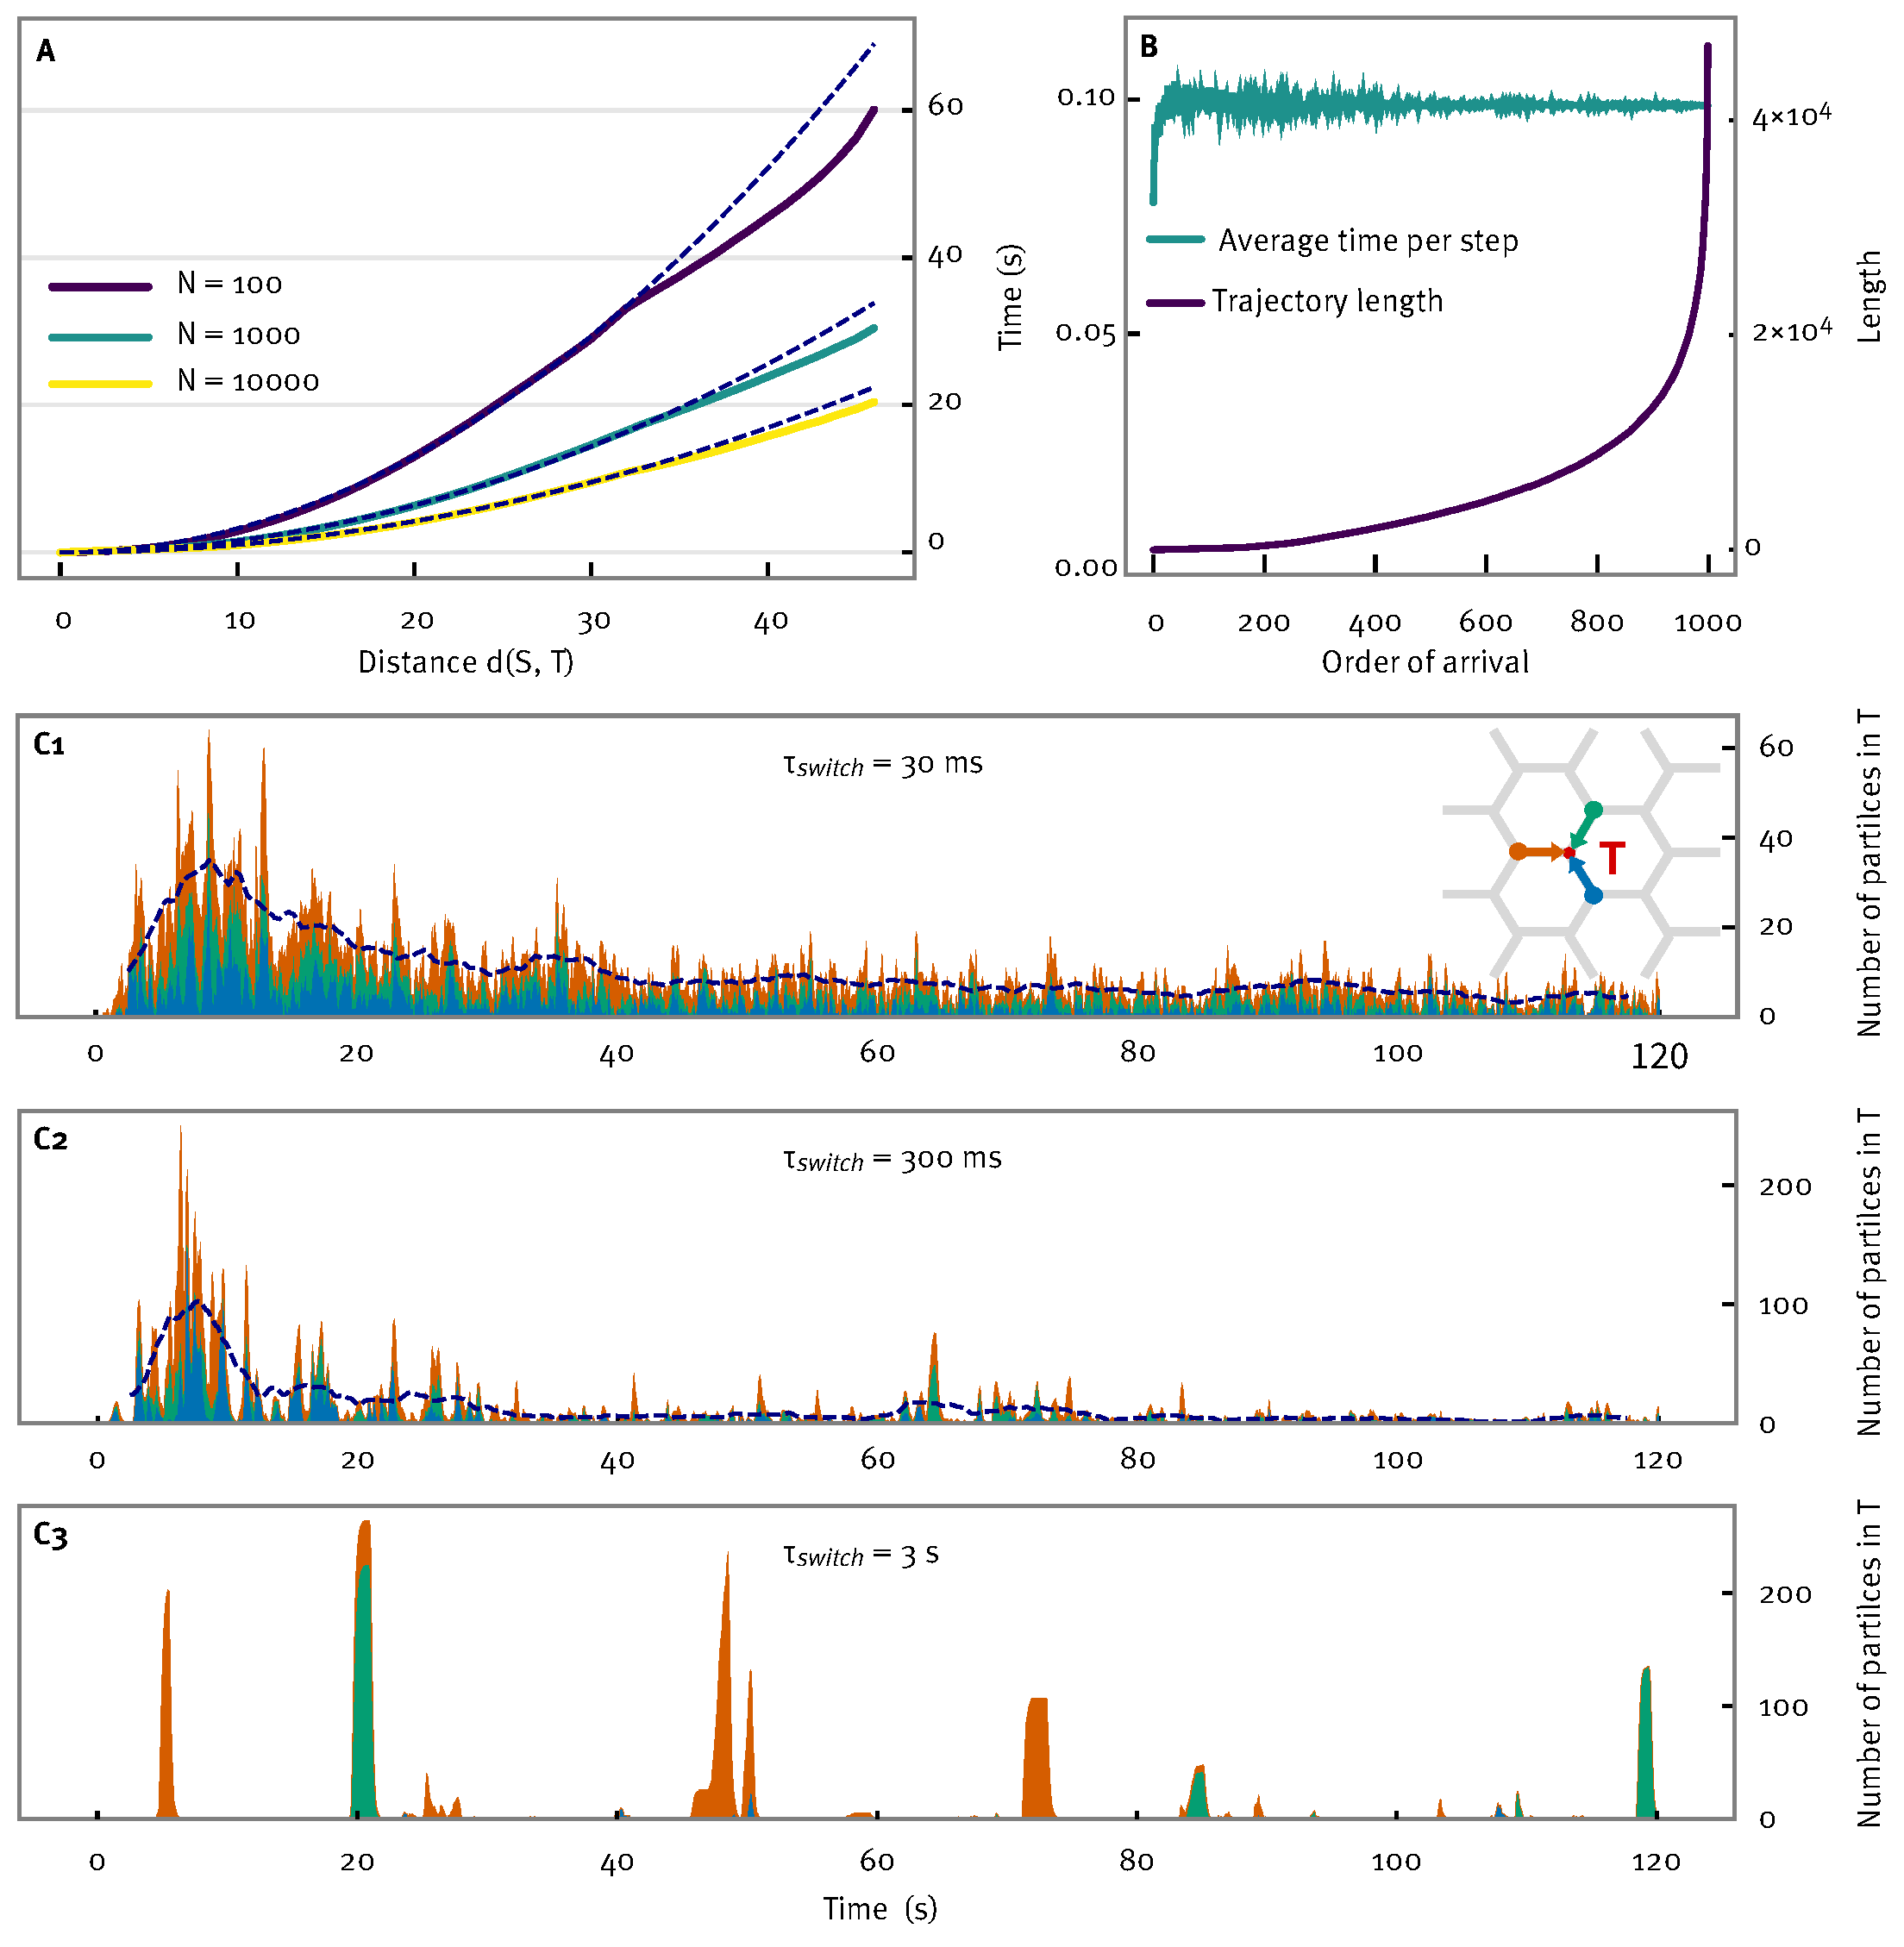
\includegraphics[width=186mm]{er/3_extremes.eps}%
    {{\phantomsubcaption{}\label{fig:ex_efpt}}%
    {\phantomsubcaption{}\label{fig:ex_traj}}%
    {\phantomsubcaption{}\label{fig:ex_packet}}}%
    \caption{Extremes statistics and packet motion.
    \subref{fig:ex_efpt}\enspace \tsc{EFPT} (time for the first to arrive( on the hexagonal network for different values of N (total number of particles). The dashed line shows the fit for $c_1 \frac{\delta^2}{c_2 + \log N}$ with $c_1 = 0.07$ and $c_2 = -2.39$. \subref{fig:ex_traj}\enspace characteristics of the trajectories by order of arrival (1000 out of 10⁴ trajectories are considered). The plot shows how the trajectory length has a greater impact on the time to arrive than a deviation from the mean time per step.
    \subref{fig:ex_packet}\enspace number of particles in a target node T as a function of time. The area plot is coloured based on the edge particles are coming from. For small values of $\tau_{switch}$, an uniform equilibrium distribution is reached after large enough time (figs. C1--2). Instead, for slow switching, a new kind of motion emerges. Particles arrive in the node in lumps (\emph{packets}), at random times (fig. C3).\label{fig:ex}}
  \end{adjustwidth*}
\end{figure}

\section{Packet motion}

In a standard random walk on a graph, the probability of finding the walker in a given node at equilibrium tends to an uniform distribution\mcite{lovasz1993random}. This means that if we release a group of particles from a source, given a sufficiently long time, they will distribute evenly on the network with a timescale proportional to the largest eigenvalue of the stochastic matrix representing the transition probabilities between nodes. What happens instead on the active network model? When considering a fast edge switching rate ($\tau_{switch}$ = \SIrange{30}{300}{\milli\second}), the equilibrium behaviour is preserved, leading to a roughly constant number of particles per node (figs. \ref{fig:ex_packet}1--2). For a slow switching timescale instead ($\tau_{switch} = \SI{3}{\second}$), a novel mechanism of transport emerges. Particles group in lumps, synchronising their motion and arriving in nodes in \emph{packets} (see \cref{fig:ex_packet}3). These packets are not stable: they are continuously formed (and unpacked) by splitting and merging of different particles or smaller packets. This behaviour undermine the realisation of a even distribution, as the edge switching keeps the system out of equilibrium. This mechanism allows for a delivery in redundant groups, which seems a way to guarantee robustness to a biological transport process.
